\documentclass{beamer}
\mode<presentation>{
  \usetheme{Boadilla}
  \usefonttheme[onlylarge]{structurebold}
  \usefonttheme[stillsansseriflarge]{serif}
  \setbeamerfont*{frametitle}{size=\normalsize,series=\bfseries}
  % \setbeamertemplate{navigation symbols}{}
  \setbeamercovered{transparent}
}
\usepackage[english]{babel}
\usepackage[latin1]{inputenc}
\usepackage{times}
\usepackage[T1]{fontenc}
\usepackage{amsmath}
\usepackage{amssymb}
\usepackage{esint}
\usepackage{hyperref}
\usepackage{tikz}
\usepackage{xkeyval}
\usepackage{xargs}
\usepackage{verbatim}
\usepackage{listings}
\usepackage{multimedia}
\usepackage{bm}
\usepackage{siunitx}
\usetikzlibrary{
  arrows,
  calc,
  decorations.pathmorphing,
  decorations.pathreplacing,
  decorations.markings,
  fadings,
  positioning,
  shapes,
  arrows.meta
}
\usepgfmodule{oo}

\pgfdeclareradialshading{glow2}{\pgfpoint{0cm}{0cm}}{
  color(0mm)=(white);
  color(2mm)=(white);
  color(8mm)=(black);
  color(10mm)=(black)
}
\pgfdeclareradialshading{glow}{\pgfpoint{0cm}{0cm}}{
  color(0mm)=(white);
  color(5mm)=(white);
  color(9mm)=(black);
  color(10mm)=(black)
}

\begin{tikzfadingfrompicture}[name=glow fading]
  \shade [shading=glow] (0,0) circle (1);
\end{tikzfadingfrompicture}

\begin{tikzfadingfrompicture}[name=glow2 fading]
  \shade [shading=glow2] (0,0) circle (1);
\end{tikzfadingfrompicture}

\mode<handout>{
  \usepackage{pgfpages}
  \pgfpagesuselayout{4 on 1}[a4paper,landscape,border shrink=5mm]
  \setbeamercolor{background canvas}{bg=black!10}
}

\newcommand\pgfmathsinandcos[3]{%
  \pgfmathsetmacro#1{sin(#3)}%
  \pgfmathsetmacro#2{cos(#3)}%
}
\newcommand\LongitudePlane[3][current plane]{%
  \pgfmathsinandcos\sinEl\cosEl{#2} % elevation
  \pgfmathsinandcos\sint\cost{#3} % azimuth
  \tikzset{#1/.estyle={cm={\cost,\sint*\sinEl,0,\cosEl,(0,0)}}}
}
\newcommand\LatitudePlane[3][current plane]{%
  \pgfmathsinandcos\sinEl\cosEl{#2} % elevation
  \pgfmathsinandcos\sint\cost{#3} % latitude
  \pgfmathsetmacro\yshift{\cosEl*\sint}
  \tikzset{#1/.estyle={cm={\cost,0,0,\cost*\sinEl,(0,\yshift)}}} %
}
\newcommand\DrawLongitudeCircle[2][1]{
  \LongitudePlane{\angEl}{#2}
  \tikzset{current plane/.prefix style={scale=#1}}
  % angle of "visibility"
  \pgfmathsetmacro\angVis{atan(sin(#2)*cos(\angEl)/sin(\angEl))} %
  \draw[current plane] (\angVis:1) arc (\angVis:\angVis+180:1);
  \draw[current plane,dashed] (\angVis-180:1) arc (\angVis-180:\angVis:1);
}
\newcommand\DrawLatitudeCircleArrow[2][1]{
  \LatitudePlane{\angEl}{#2}
  \tikzset{current plane/.prefix style={scale=#1}}
  \pgfmathsetmacro\sinVis{sin(#2)/cos(#2)*sin(\angEl)/cos(\angEl)}
  % angle of "visibility"
  \pgfmathsetmacro\angVis{asin(min(1,max(\sinVis,-1)))}
  \draw[current plane,decoration={markings, mark=at position 0.6 with {\arrow{<}}},postaction={decorate},line width=.6mm] (\angVis:1) arc (\angVis:-\angVis-180:1);
  \draw[current plane,dashed,line width=.6mm] (180-\angVis:1) arc (180-\angVis:\angVis:1);
}
\newcommand\DrawLatitudeCircle[2][1]{
  \LatitudePlane{\angEl}{#2}
  \tikzset{current plane/.prefix style={scale=#1}}
  \pgfmathsetmacro\sinVis{sin(#2)/cos(#2)*sin(\angEl)/cos(\angEl)}
  % angle of "visibility"
  \pgfmathsetmacro\angVis{asin(min(1,max(\sinVis,-1)))}
  \draw[current plane] (\angVis:1) arc (\angVis:-\angVis-180:1);
  \draw[current plane,dashed] (180-\angVis:1) arc (180-\angVis:\angVis:1);
}
\newcommand\coil[1]{
  {\rh * cos(\t * pi r)}, {\apart * (2 * #1 + \t) + \rv * sin(\t * pi r)}
}
\makeatletter
\define@key{DrawFromCenter}{style}[{->}]{
  \tikzset{DrawFromCenterPlane/.style={#1}}
}
\define@key{DrawFromCenter}{r}[1]{
  \def\@R{#1}
}
\define@key{DrawFromCenter}{center}[(0, 0)]{
  \def\@Center{#1}
}
\define@key{DrawFromCenter}{theta}[0]{
  \def\@Theta{#1}
}
\define@key{DrawFromCenter}{phi}[0]{
  \def\@Phi{#1}
}
\presetkeys{DrawFromCenter}{style, r, center, theta, phi}{}
\newcommand*\DrawFromCenter[1][]{
  \setkeys{DrawFromCenter}{#1}{
    \pgfmathsinandcos\sint\cost{\@Theta}
    \pgfmathsinandcos\sinp\cosp{\@Phi}
    \pgfmathsinandcos\sinA\cosA{\angEl}
    \pgfmathsetmacro\DX{\@R*\cost*\cosp}
    \pgfmathsetmacro\DY{\@R*(\cost*\sinp*\sinA+\sint*\cosA)}
    \draw[DrawFromCenterPlane] \@Center -- ++(\DX, \DY);
  }
}
\newcommand*\DrawFromCenterText[2][]{
  \setkeys{DrawFromCenter}{#1}{
    \pgfmathsinandcos\sint\cost{\@Theta}
    \pgfmathsinandcos\sinp\cosp{\@Phi}
    \pgfmathsinandcos\sinA\cosA{\angEl}
    \pgfmathsetmacro\DX{\@R*\cost*\cosp}
    \pgfmathsetmacro\DY{\@R*(\cost*\sinp*\sinA+\sint*\cosA)}
    \draw[DrawFromCenterPlane] \@Center -- ++(\DX, \DY) node {#2};
  }
}
\makeatother

% not mandatory, but I though it was better to set it blank
\setbeamertemplate{headline}{}
\def\beamer@entrycode{\vspace{-\headheight}}

\tikzstyle{snakearrow} = [decorate, decoration={pre length=0.2cm,
  post length=0.2cm, snake, amplitude=.4mm,
  segment length=2mm},thick, ->]

%% document-wide tikz options and styles

\tikzset{%
  % >=latex, % option for nice arrows
  inner sep=0pt,%
  outer sep=2pt,%
  mark coordinate/.style={inner sep=0pt,outer sep=0pt,minimum size=3pt,
    fill=black,circle}%
}
\tikzset{
  % Define standard arrow tip
  >=stealth',
  % Define style for boxes
  punkt/.style={
    rectangle,
    rounded corners,
    draw=black, very thick,
    text width=8em,
    minimum height=2.5em,
    text centered},
}
\makeatletter
\newbox\@backgroundblock
\newenvironment{backgroundblock}[2]{%
  \global\setbox\@backgroundblock=\vbox\bgroup%
  \unvbox\@backgroundblock%
  \vbox to0pt\bgroup\vskip#2\hbox to0pt\bgroup\hskip#1\relax%
}{\egroup\egroup\egroup}
\addtobeamertemplate{background}{\box\@backgroundblock}{}
\makeatother

% Steps
%% Cooling molecule is hard.
%% In order to reach the ultra cold temperature needed for, assemble from atoms instead.
%% Start from two atoms grab from MOT (pic)
%% Do Raman sideband cooling (spectrum, performance)
%% Merge and make molecules (merge graph?)

% Making molecules with optical transitions
%% Wavefunction size difference
%% Use an intermediate state to bridge the difference

% Finding the excited state

% EIT scan

% \def\timeleft{15:00->14:55}

\title[NaCs in optical tweezer]{Observation of NaCs molecular state in optical tweezer}
\date{April 04, 2018}
\author[Yichao Yu]{Yichao Yu\\
  \vspace{0.5cm}
  {\footnotesize Lee Liu, Dr. Jon Hood}}
\institute{Ni Group/Harvard}

\begin{document}


% Title
%% Talk about how we'll make NaCs molecules in optical tweezers

{
  \usebackgroundtemplate{
    \makebox[\paperwidth][c]{\centering\includegraphics[height=\paperheight]{front_bg.png}}
  }
  \setbeamercolor{title}{fg=cyan!30}
  \setbeamercolor{author}{fg=white}
  \setbeamercolor{institute}{fg=white}
  \setbeamercolor{date}{fg=white}
  \begin{frame}{}
    \titlepage
  \end{frame}
}

% \begin{frame}{}
%   \tableofcontents
% \end{frame}

\pgfdeclarelayer{tweezer}
\pgfsetlayers{tweezer,main}
\pgfooclass{tweezer}{
  \method tweezer() {
  }
  \method drawTweezer(#1,#2,#3) {
    \begin{pgfonlayer}{tweezer}
      \shade[shading=radial,path fading=glow fading,shift={(#1,#2)},rotate=90,yscale=1,
      fill opacity=0.9,inner color=#3]
      plot[draw,samples=200,domain=-2.5:2.5] function {sqrt(0.01 + x**2 / 10)}
      -- plot[draw,samples=200,domain=2.5:-2.5] function {-sqrt(0.01 + x**2 / 10)};
    \end{pgfonlayer}
  }
  \method drawAtom(#1,#2,#3,#4) {
    \fill [#4,path fading=glow2 fading] (#1,#2) circle (#3);
  }
  \method drawNaAtom(#1,#2,#3) {
    \pgfoothis.drawAtom(#1,#2,#3,blue);
  }
  \method drawCsAtom(#1,#2,#3) {
    \pgfoothis.drawAtom(#1,#2,#3,red);
  }
  \method drawNaTweezer(#1,#2) {
    \pgfoothis.drawTweezer(#1,#2,blue!35!black!30);
  }
  \method drawCsTweezer(#1,#2) {
    \pgfoothis.drawTweezer(#1,#2,red!30!black!30);
  }
  \method up(#1,#2) {
    \pgfoothis.drawCsTweezer(#1,#2);
    \pgfoothis.drawNaAtom(#1,#2+0.06,0.12);
    \pgfoothis.drawCsAtom(#1,#2-0.06,0.16);
  }
  \method down(#1,#2) {
    \pgfoothis.drawCsTweezer(#1,#2);
    \pgfoothis.drawCsAtom(#1,#2+0.06,0.16);
    \pgfoothis.drawNaAtom(#1,#2-0.06,0.12);
  }
  \method naTrap(#1,#2) {
    \pgfoothis.drawNaTweezer(#1,#2);
    \pgfoothis.drawNaAtom(#1,#2,0.12);
  }
  \method csTrap(#1,#2) {
    \pgfoothis.drawCsTweezer(#1,#2);
    \pgfoothis.drawCsAtom(#1,#2,0.16);
  }
}
\pgfoonew \mytweezer=new tweezer()

% Goal
%% Single dipolar molecules in an array of optical tweezers.
%% Combining the ...(internal state, tunable long range interaction)... of dipolar molecules
%% And precise manipulation and detection capability of optical tweezers
%% Promissing system to do quantum simulation/computation/chemistry
%% Molecule of choise is NaCs, strong dipole moment and easy to cool.

\begin{frame}{}
  \begin{center}
    \begin{tikzpicture}[scale=0.75]
      \mytweezer.up(0, 0)
      \mytweezer.down(2, 0.8/2.5)
      \mytweezer.up(4, 1.2/2.5)
      \begin{pgfonlayer}{tweezer}
        \draw[line width=1,dashed,color=cyan] (0, 0/2.5) -- (2, 0.8/2.5);
        \draw[line width=1,dashed,color=cyan] (0, 0/2.5) -- (1, -1.7/2.5);
        \draw[line width=1,dashed,color=cyan] (2, 0.8/2.5) -- (1, -1.7/2.5);
        \draw[line width=1,dashed,color=cyan] (3, -2.1/2.5) -- (1, -1.7/2.5);
        \draw[line width=1,dashed,color=cyan] (3, -2.1/2.5) -- (2, 0.8/2.5);
        \draw[line width=1,dashed,color=cyan] (4, 1.2/2.5) -- (2, 0.8/2.5);
        \draw[line width=1,dashed,color=cyan] (3, -2.1/2.5) -- (4, 1.2/2.5);
        \draw[line width=1,dashed,color=cyan] (3, -2.1/2.5) -- (5, -1.9/2.5);
        \draw[line width=1,dashed,color=cyan] (4, 1.2/2.5) -- (5, -1.9/2.5);
        \draw[line width=1,dashed,color=cyan] (6.2, -0.9/2.5) -- (4, 1.2/2.5);
        \draw[line width=1,dashed,color=cyan] (6.2, -0.9/2.5) -- (5, -1.9/2.5);
      \end{pgfonlayer}
      \mytweezer.down(1, -1.7/2.5)
      \mytweezer.up(3, -2.1/2.5)
      \mytweezer.down(5, -1.9/2.5)
      \mytweezer.down(6.2, -0.9/2.5)
      \visible<2>{
        \fill[white,opacity=0.4] (-0.8, -4) rectangle (9, 3);
      }
      \visible<3>{
        \fill[white,opacity=0.8] (-0.8, -4) rectangle (9, 3);
        \node[align=center] at (3, 0) {{\textbf{\huge NaCs}}\\\\
          \Large Dipole moment: $4.6\ \mathrm{Debye}$};
      }
      \visible<2->{
        \node at (3, -6) {\includegraphics[width=5.5cm]{quantum_simulation.png}};
        \node at (10.5, -0.5) {\includegraphics[height=5cm]{quantum_chemistry.pdf}};
        \node at (10.5, -6.5) {\includegraphics[width=6.5cm]{quantum_computing.pdf}};
      }
    \end{tikzpicture}
  \end{center}
\end{frame}

\begin{frame}{}
\end{frame}

% \begin{frame}{Wave function size mismatch}
%   \begin{center}
%     \begin{tikzpicture}
%       \shade[ball color=blue!90] (0, 0) circle (0.45);
%       \shade[ball color=orange!90] (0.4, 0.2) circle (0.3);
%       \draw[<->,line width=1] (-0.45, 0.4) -- (0.35, 0.8);
%       \path (-0.05, 0.6) node[rotate=26.565,above=2pt] {$4a_0$};
%       \path (0.2, -2) node[below] {\textbf{Molecule}};

%       \draw[line width=1] plot[samples=200,domain=-2:2,variable=\x] ({\x + 6}, {(\x)^2 * 0.8 - 1.5});
%       \draw[line width=2,orange!90!black]
%       plot[samples=200,domain=-2:2,variable=\x] ({\x + 6}, {exp(-(\x)^2 * 1.3) - 0.988});
%       \draw[line width=0.8] (6 - 0.8, -0.988) -- (6 + 0.8, -0.988);
%       \draw[<->,line width=1] (6 - 1, 0.3) -- (6 + 1, 0.3);
%       \path (6, 0.3) node[above] {$1000a_0$};
%       \path (6, -2) node[below] {\textbf{Atom}};
%     \end{tikzpicture}
%     \vspace{1cm}
%     \begin{block}{Goal of cooling}
%       \begin{itemize}
%       \item Single initial state
%       \item Shrink wavefunction size
%       \end{itemize}
%     \end{block}
%   \end{center}
% \end{frame}

% \begin{frame}{Raman sideband cooling of Sodium}
%   \begin{columns}
%     \column{6.5cm}
%     % 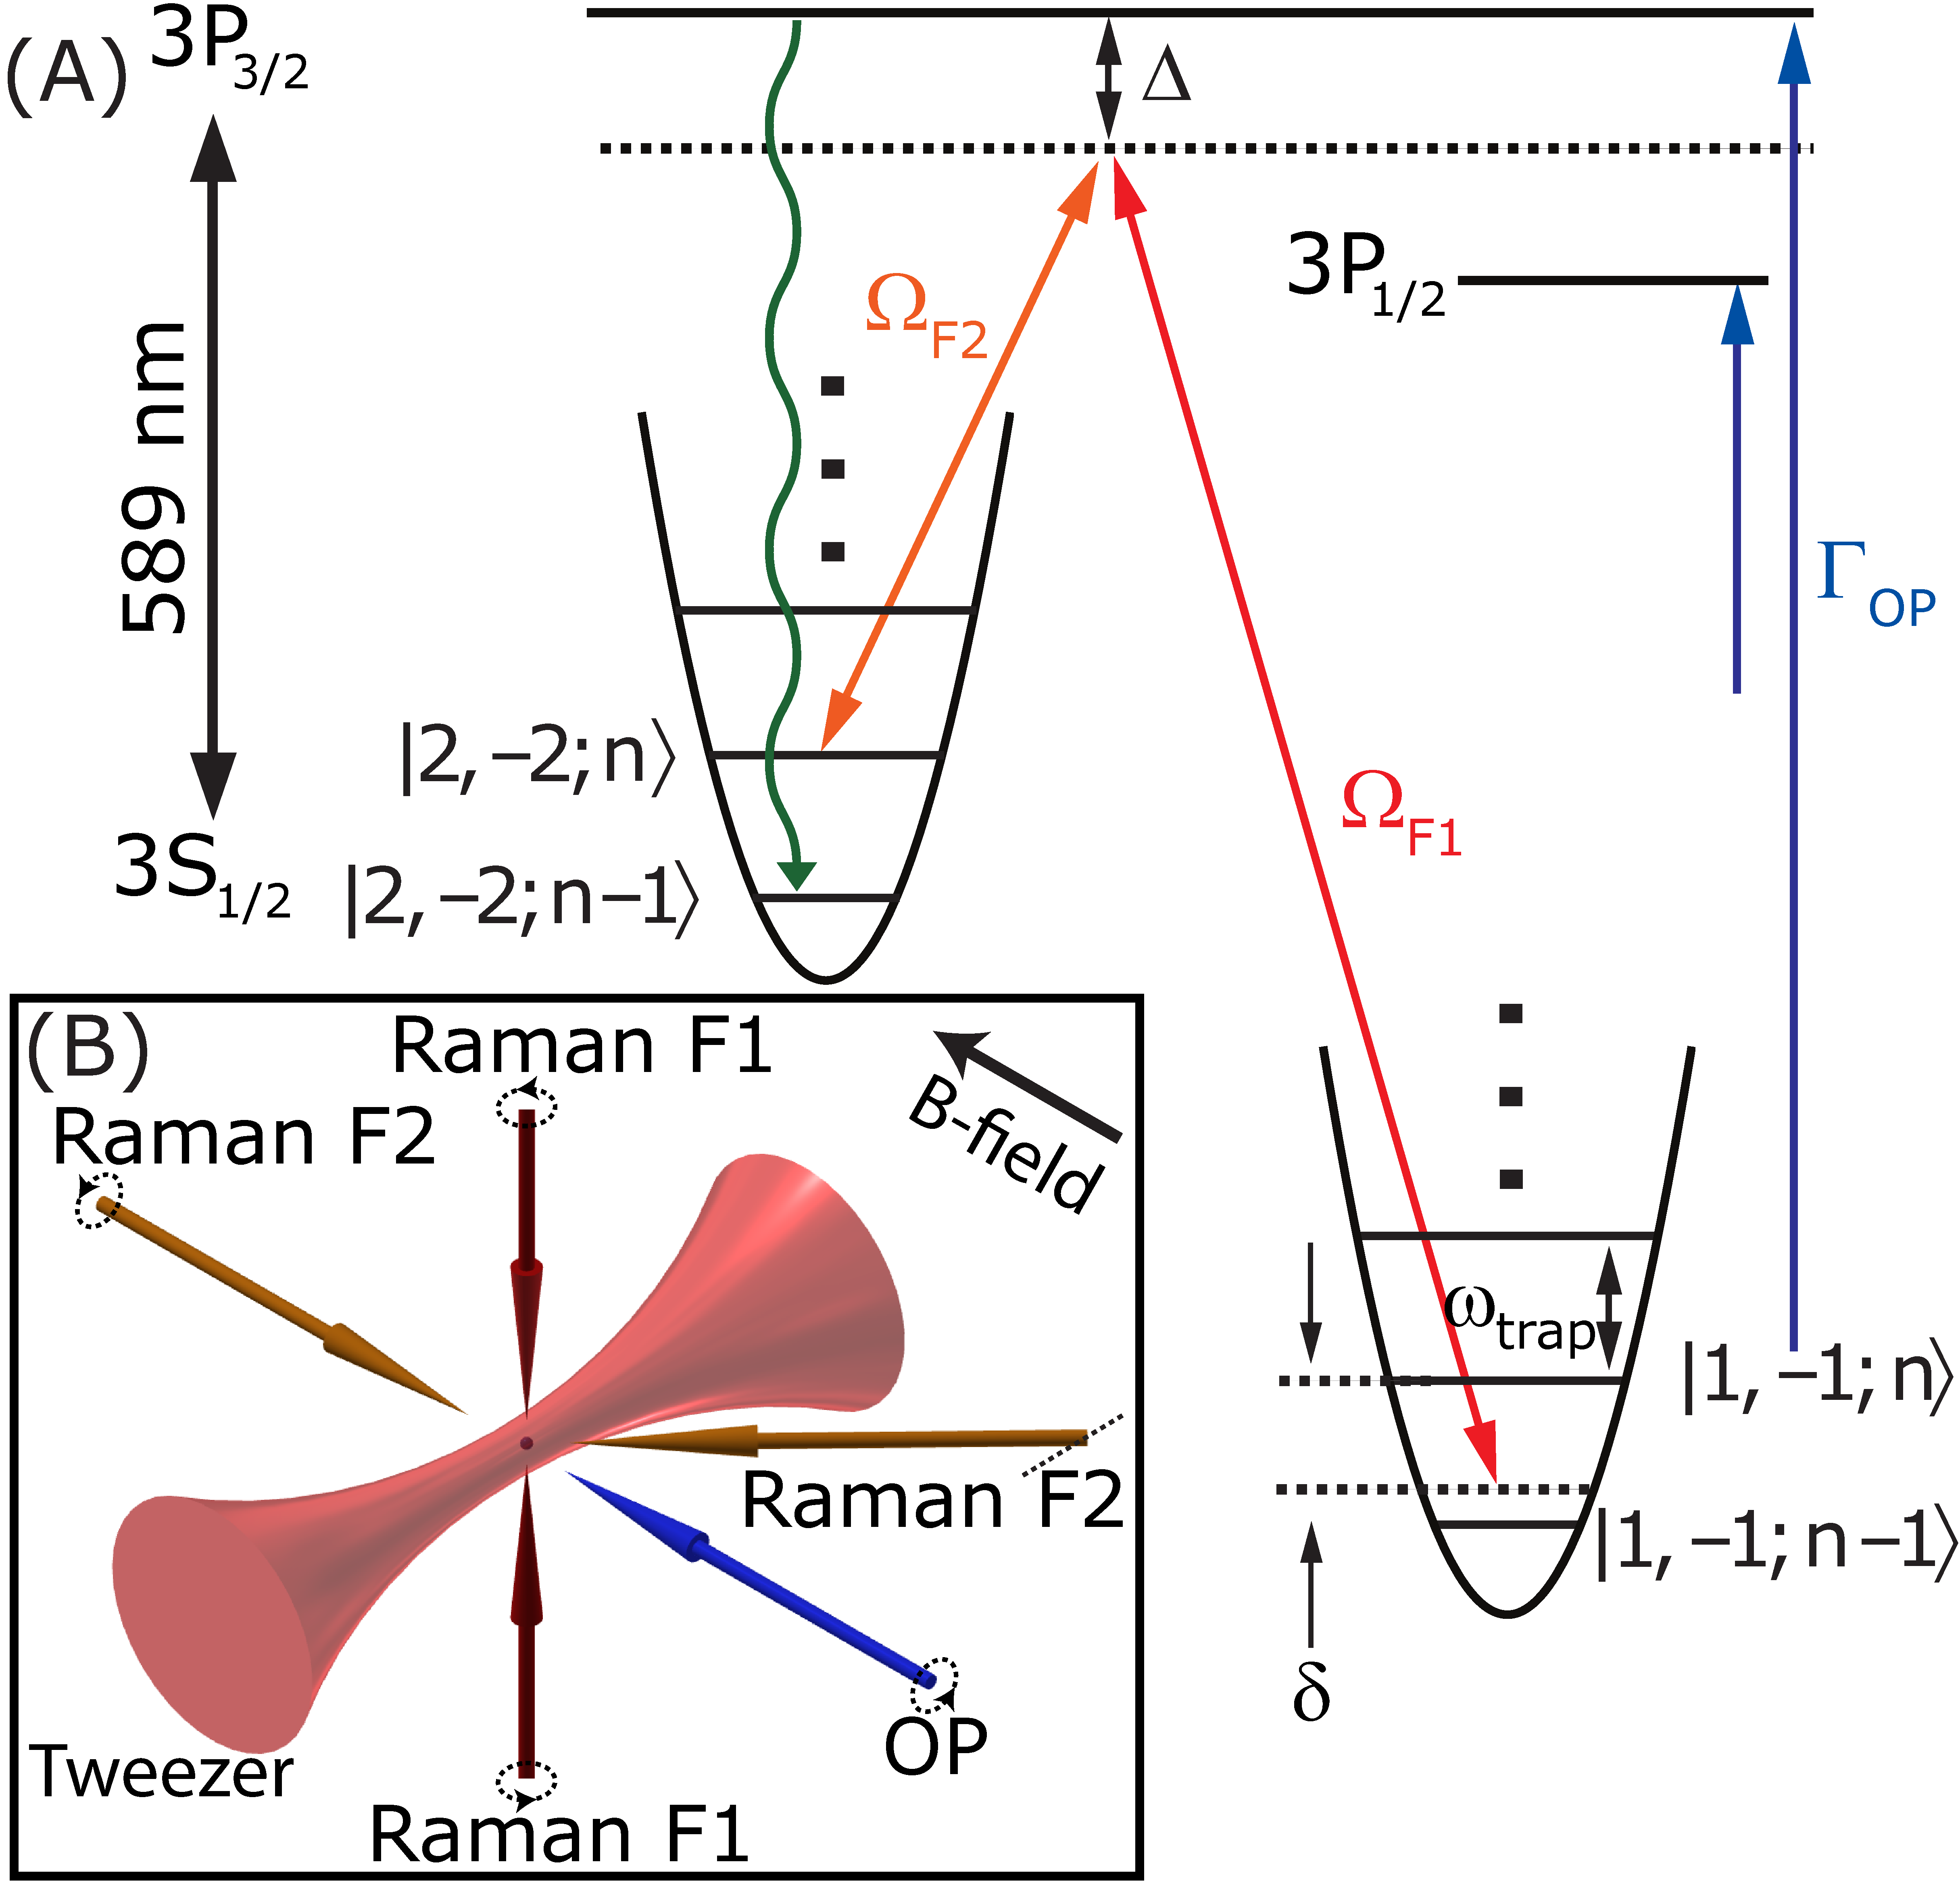
\includegraphics[width=6cm]{Na_RSC_schematic.pdf}
%     \column{5cm}
%     \visible<2->{
%       \begin{block}{Difficulties}
%         \begin{itemize}
%         \item High initial temperature ($40\mu K$)
%         \item<3-> High recoil heating\\
%           {\footnotesize (High Lamb Dicke parameter)}
%         \end{itemize}
%       \end{block}
%     }
%   \end{columns}
% \end{frame}

% \begin{frame}{Raman sidebands}
%   \begin{center}
%     \begin{tikzpicture}
%       \visible<1> {
%         \path (0, 0) node {
%           \includegraphics[width=10cm]{../../experiments/misc/imgs/data_spectrum_20170409_r2_before.png}
%         };
%         \draw[<-, line width=1.5] (-0.7, 0) -- (0, 1.6) node[right] {\Large Carrier};
%       }
%       \visible<2> {
%         \path (0, 0) node {
%           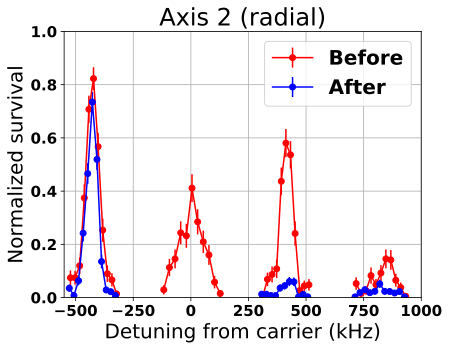
\includegraphics[width=10cm]{../../experiments/misc/imgs/data_spectrum_20170409_r2.png}
%         };
%       }
%       \visible<3> {
%         \path (0, 0) node {
%           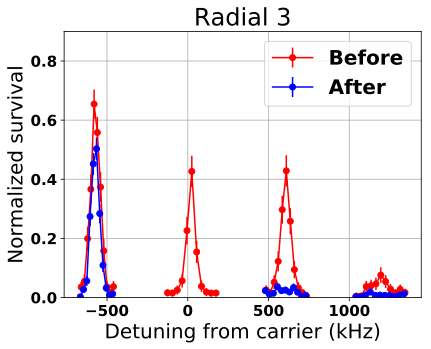
\includegraphics[width=10cm]{../../experiments/misc/imgs/data_spectrum_20170409_r3.png}
%         };
%       }
%     \end{tikzpicture}
%   \end{center}
% \end{frame}

% \begin{frame}{Raman sidebands}
%   \begin{center}
%     \begin{tikzpicture}[scale=1.41176]
%       \visible<1> {
%         \path (0, 0) node {
%           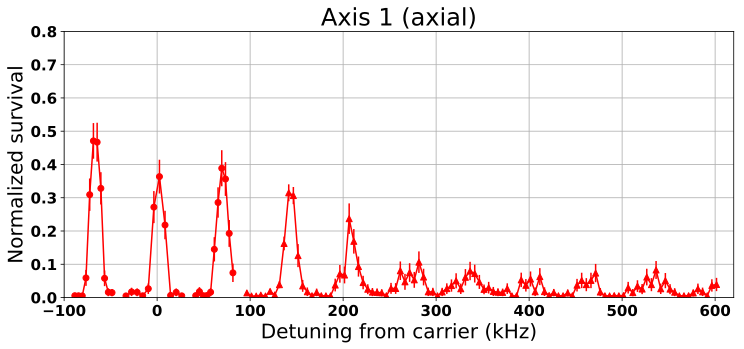
\includegraphics[width=12cm]{../../experiments/misc/imgs/data_spectrum_20170409_a1_before.png}
%         };
%         \draw[red, <-, line width=1.5] (-3.15, 0.5) -- (-2.95, 1.2)
%         node[above right] {\Large 1st order heating};
%         \draw[<-, line width=1.5] (-2.45, 0.2) -- (-2.25, 0.8) node[above right] {\Large Carrier};
%         \draw[black!40!green, <-, line width=1.5] (-1.7, 0.2) -- (-1.55, 0.6)
%         node[right] {\Large 1st order cooling};
%         \draw[blue, <-, line width=1.5] (-0.95, -0.1) -- (-0.55, 0.1)
%         node[right] {\Large 2nd order cooling};
%         \path[magenta] (0.25, -0.5) node[right] {\Large And higher orders{$\cdots$}};
%       }
%       \visible<2-> {
%         \path (0, 0) node {
%           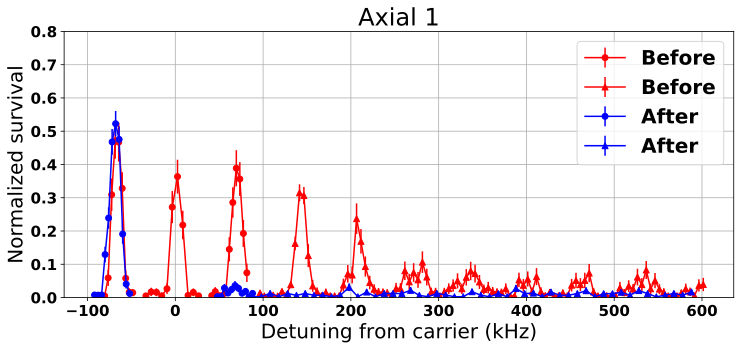
\includegraphics[width=12cm]{../../experiments/misc/imgs/data_spectrum_20170409_a1.png}
%         };
%       }
%       \visible<3-> {
%         \fill[white,opacity=0.95] (-4.2, -2.5) rectangle (5, 2.5);
%         \path (0, 1) node[align=center]
%         {
%           \begin{tabular}{|c|c|}
%             \hline
%             \textbf{Axis}&\textbf{Ground state probability}\\\hline
%             1 (Axial)&93.1(2.5)\%\\\hline
%             2 (Radial)&91.9(2.3)\%\\\hline
%             3 (Radial)&92.9(2.5)\%\\\hline
%           \end{tabular}
%         };
%         \visible<4-> {
%           \path (0, -1) node[align=center]
%           {
%             \textbf{3D ground state:} $79.5(3.6)\%$\\
%             \textbf{Loss after cooling:} $15\%$\\\\
%             \textbf{Total 3D ground state preparation fidelity:} $67.6(3.1)\%$
%           };
%         }
%       }
%     \end{tikzpicture}
%   \end{center}
% \end{frame}

% \begin{frame}{Rabi flopping (radial)}
%   \begin{center}
%     \visible<+->{
%       \includegraphics[width=10cm]{../../experiments/rabi_flop/imgs/fit_20170409_r2_0_ba.png}\\
%     }
%     \visible<+->{
%       Good agreement in ground state probability between spectrum and Rabi flopping data.
%     }
%   \end{center}
% \end{frame}

% \begin{frame}{Rabi flopping (axial)}
%   \begin{center}
%     \includegraphics[height=4.8cm]{../../experiments/rabi_flop/imgs/fit_20170409_a1_0_nol.png}
%     \includegraphics[height=4.8cm]{../../experiments/rabi_flop/imgs/fit_20170409_a1_p1_nol.png}
%   \end{center}
% \end{frame}

% \begin{frame}{}
%   \begin{block}{Conclusion}
%     $67.6(3.1)\%$ ground state preparation fidelity {\small ($79.5(3.6)\%$ without loss)}
%   \end{block}
%   \vspace{1cm}
%   \begin{block}{Improvements}
%     \begin{itemize}
%     \item Reduce off-resonance scattering from Raman beams
%     \item Reduce magnetic field fluctuation
%     \item Reduce loss during cooling
%     \end{itemize}
%   \end{block}
% \end{frame}

% \begin{frame}{}
% \end{frame}

% \begin{frame}{Axial matrix element}
%   \begin{center}
%     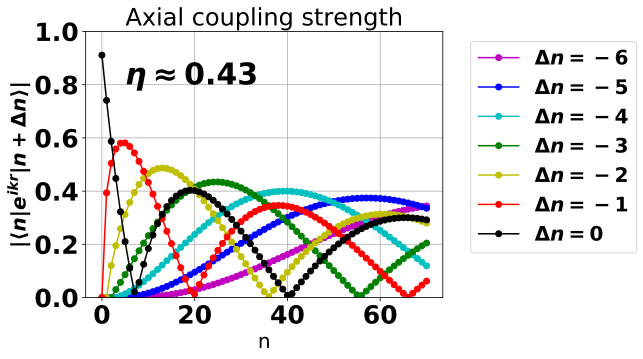
\includegraphics[width=6.5cm]{{../../calculations/sideband_strength/imgs/coupling_0.43_0-6}.png}
%   \end{center}
% \end{frame}

% \begin{frame}{Radial 2 matrix element}
%   \begin{center}
%     \includegraphics[width=6.5cm]{{../../calculations/sideband_strength/imgs/coupling_0.35_0-2}.png}
%   \end{center}
% \end{frame}

% \begin{frame}{Radial 3 matrix element}
%   \begin{center}
%     \includegraphics[width=6.5cm]{{../../calculations/sideband_strength/imgs/coupling_0.29_0-2}.png}
%   \end{center}
% \end{frame}

\end{document}
